\section{Parallel coordinate descent methods}\label{pcdm}
We demonstrated that the true $PSF$ of the deconvolution problem can be approximated. A smaller $PSF$ can be used, which is only a fraction of the true size. The serial coordinate descent methods, which was used so during this project, achieves a moderate speedup with the $PSF$ approximation. Parallel coordinate descent methods may benefit more from the $PSF$ approximation. For the rest of this work, we develop a parallel coordinate descent deconvolution algorithm. We explain why parallel methods should benefit more from the $PSF$ approximation, and show that they indeed speed up the deconvolution problem.


Introduce the principle of parallel coordinate descent methods, and derrive a parallel coordinate descent deconvolution algorithm.

%Naive way to exploit this, we can create patches of the image, four of which are independent of each other.
%Deconvolve four patches in parallel.
%Work is not equally distributed on the different patches. 



\subsection{From serial to parallel}
Parallel coordinate descent methods take several steps at different coordinates before they update the gradient map. The difficulty in parallel coordinate descent methods lies in dealing with correlated pixel values> In our deconvolution problem, two pixels which are close to each other in the image are correlated. The more they overlap, the more we over-estimate their pixel values with parallel coordinate descent methods\footnote{Imagine we optimize two pixels next to each other in serial coordinate descent: The serial coordinate descent algorithm  optimizes he first pixel, updates the gradient, and then optimizes the second pixel. The value of the second pixel will be magnitudes lower than the first, because most of the emission in that area was already explained by the first pixel. If however we update in parallel, both pixels will end up with a similar value, and both pixels try to explain the same emission.}. This over-estimation leads to slow convergence. Or if we increase the number of parallel updates, can lead to a divergence. This means we cannot simply modify our serial coordinate descent algorithm to take a number of parallel steps. We need a way to deal with the over-estimation. 

Our serial coordinate descent algorithm uses a greedy pixel selection strategy. Parallel coordinate descent methods on the other hand often select their pixels uniformly at random. The random selection strategy lets us estimate how much the parallel algorithm over-estimates the pixel values\cite{richtarik2016parallel}. However, a random strategy is not efficient for our deconvolution problem.

We first explain the parallel coordinate descent method in the next section \ref{pcdm:pcdm}. We then introduce the modifications we developed for an efficient parallel deconvolution algorithm.

%Parallel coordinate descent methods have a strategy to deal with correlated pixel values: The shotgun algorithm\cite{bradley2011parallel} estimates the number parallel random updates that can be taken without diverging. PCDM estimates the expected $PSF$ overlap between random pixels, and adjusts the step size accordingly. In this project, we use the PCDM algorithm and its accelerated variant APPROX \cite{fercoq2015accelerated}. We introduce the algorithm in Section \ref{pcdm:pcdm}.

%Note that parallel coordinate descent methods tend to select pixels at random. This helps dealing with correlated pixel values: In our deconvolution case, the pixels which are close by to each other tend to be correlated more strongly. But the exact shape of the $PSF$ is also a factor. If the $PSF$s overlap only in a region where it is close to zero, the pair of pixels also have a low correlation factor. A random selection strategy helps to keep a low correlation factor on average, no matter what the $PSF$ looks like. 

%But for our deconvolution case, a random strategy brings in its own issues. Remember that the LMC has a bright supernova remnant N132D, which overshadows other sources. A deconvolution algorithm has to deconvolve the pixels belonging to N132D first. A random strategy may waste resources until it has deconvolved the fairly small subset of pixels belonging to N132D. We have adapted the PCDM algorithm for the deconvolution problem, and describe our adaption in detail in Section  \ref{pcdm:adaption}.

\subsection{Parallel (Block) Coordinate Descent Method (PCDM)} \label{pcdm:pcdm}
The PCDM algorithm can be seen as a generalization of our serial coordinate descent algorithm from Section \ref{cd}. The serial algorithm optimizes a single pixel at a time. PCDM can update one, or a whole block of pixels at each iteration. And as the name implies, it can update multiple blocks of pixels in parallel. In this project, we use the accelerated variant of the PCDM algorithm, named APPROX \cite{fercoq2015accelerated}. We first introduce a PCDM deconvolution algorithm and then describe the accelerated variant.

\subsubsection{Block coordinate descent deconvolution}
Here we introduce the serial block coordinate descent algorithm. Instead of optimizing a single pixel in each iteration, the serial block coordinate descent algorithm can update a block of pixels. The block size is left for the user to define. It can be any number between a single pixel, in which case the algorithm is identical to the serial coordinate descent algorithm from Section \ref{cd}, or the whole image.

Remember the single pixel update from the serial coordinate descent algorithm: 
\begin{equation} \label{pcdm:pcdm:block:single:update}
pixel_{opt} = \frac{max(gradient_{location} - \lambda\alpha, 0)}{Lipschitz_{location} + (1 - \alpha)\lambda}
\end{equation}

We optimize the pixel at the current location by taking the gradient and dividing it by the Lipschitz constant. For the serial block coordinate descent algorithm we vectorize the update rule. That means $gradient_{location}$ and $Lipschitz_{location}$ and the output $pixel_{opt}$ become vectors:

\begin{equation} \label{pcdm:pcdm:block:block:update}
pixels_{opt} = \frac{max(gradients_{locations} - \lambda\alpha, 0)}{Sum(Lipschitz_{locations}) + (1 - \alpha)\lambda}
\end{equation}

This is the serial block coordinate descent update rule. Note that we divide the gradient for each pixel by the the block Lipschitz constant (which is the sum of every pixel Lipschitz constant in the block). The single pixel update rule can take a larger step, but only for a single pixel. 

The reader might be familiar with the (F)ISTA method\cite{beck2009fista}. The block update shown in equation \eqref{pcdm:pcdm:block:block:update} is related to the (F)ISTA update step. When the block size equal to the image size (we update all pixels in the image in each iteration), then the serial block coordinate descent is equivalent to (F)ISTA.


\subsubsection{Parallel block coordinate descent deconvolution}
We present the parallel block coordinate descent algorithm. It is based on the PCD method\cite{richtarik2016parallel}. In this section, we show how it can be used to solve the deconvolution problem. Our parallel coordinate descent algorithm updates $t$ random blocks of pixels in parallel in each iteration. Each iteration is split into three steps: Step 1 is to select $t$ unique blocks of pixels uniformly at random (we cannot select the same block multiple times). In step 2 we update in parallel each selected block in the reconstructed image $x$. And finally in step 3 we update the gradient map.

\begin{lstlisting}
dirty = IFFT(GridVisibilities(visibilities))
residualsPadded = ZeroPadding(dirty)

psfPadded = ZeroPadding(PSF)
psfPadded = FlipUD(FlipLR(psfPadded))
gradientUpdate = iFFT(FFT(ZeroPadding(PSF)) * FFT(psfPadded))

x = new Array[,]
gradientsMap = iFFT(FFT(residualsPadded) * FFT(psfPadded))
lipschitzMap = CalcLipschitz(PSF)

objectiveValue = 0.5* Sum(residuals * residuals) + ElasticNet(x)
eso = ESO(CountNonZero(PSF), t, x.Length / blockSize)

do 
	oldObjectiveValue = objectiveValue
	
	//Step 1: select t blocks uniformly at random
	blocks = sample(t)
	
	//Step 2: update reconstruction
	diffBlocks = new Array
	parallel for each block in blocks
		blockLipschitz = Sum(GetBlock(LipschitzMap, block))
		
		//increase blockLipschitz according to the ESO
		blockLipschitz = blockLipschitz * eso
		gradientsBlock = GetBlock(gradientMap, block)
		oldBlock = GetBLock(x, block)
		tmp = gradientsBlock + oldBlock * blockLipschitz
		optimalBlock = Max(tmp - lambda*alpha) / (blockLipschitz + (1 - alpha)*lambda)
		diffBlock = optimalBlock - oldBlock
		
		x[block] += diffBlock
		diffBlocks[block] = diffBlock
	
	//Step 3: Update gradients
	for each block in blocks
		diffBlock = diffBlocks[block]
		for each pixel in block
			diff = diffBlock[pixel]
			shiftedUpdate = Shift(gradientUpdate, pixelLocation)
			gradientMap = gradientMap - shiftedUpdate * diff
			
while maxAbsDiff  < epsilon
\end{lstlisting}

The parameter $t$ can be thought of as the number of processors. We select a block to optimize in parallel for each available processor. The parallel algorithm presented here is a synchronous implementation. Each processor waits for the others to finish in each step. The implementation used later in this section is asynchronous, where each processor separately selects a block, updates the reconstruction and updates the gradient map independent of the other processors. 

The core of the parallel coordinate descent algorithm is the Estimated Seperability Overapproximation (ESO). In essence, the ESO represents how much we over-estimate the pixels values when we update $t$ random blocks in parallel. To guarantee convergence, we decrease the step size by the factor of the ESO. With more processors $t$ involved, we have to take smaller and smaller steps to guarantee convergence. Here is a trade-off between the degree of parallelism and the overall convergence speed.

The ESO is derived from three components: The uniform sampling strategy used, the number of parallel updates, and the number of non-zero components in the $PSF$. We use a $t$-nice uniform sampling. The ESO that arises from the $t$-nice sampling (take $t$ blocks uniformly at random) according to\cite{richtarik2016parallel}:

\begin{equation}\label{pcdm:pcdm:eso}
ESO(\omega, t, n) = 1+ \frac{(\omega - 1)(t - 1)}{max(1, n -1)}
\end{equation}

Where $\omega$ is the number of non-zero entries in the $PSF$, $t$ is the number of parallel updates, and $n$ is the number of blocks in the problem. For example: The image is $256^2$ pixels in size, we update blocks with a size of $4^2$ pixels, the $PSF$ has $\omega = 24$ non zero entries, and we use $t = 4$ processors, then the ESO is:

\begin{equation}
ESO(\omega = 24, t = 4, n = (256^2 / 4^2)) = 1+ \frac{(24 - 1)(4 - 1)}{max(1, 4096 -1)} \approx 1.017
\end{equation}

The lowest possible value for the ESO is $1$. The fewer processors $t$ we use and the fewer non-zero components $\omega$ the $PSF$ has, the closer the ESO is to 1. We want a small ESO with the highest number of processors possible. As we see from equation \eqref{pcdm:pcdm:eso}, the ESO gets smaller with fewer non-zero values in the $PSF$.

Remember that the $PSF$ in radio astronomy is typically dense. Although most of its values are close to zero, it generally does not have any zero values. The $PSF$ approximation methods we developed in Section \ref{gradients} effectively reduce the number of non-zero values. For the parallel coordinate descent algorithm, this leads to an ESO closer to 1, even  and we can take larger steps without diverging.


\subsection{Accelerated parallel block coordinate descent method}
We introduced the parallel coordinate descent algorithm in the previous section. In this section we extend the previous algorithm with gradient acceleration, similar to the APPROX method \cite{fercoq2015accelerated}.

Instead of using a single gradient map and a single reconstructed image $x$ variable, we an 'explore' and 'correction' variable of both. The algorithm uses an $xExplore$,  $xCorrection$ and $gradientMapExplore$, $gradientMapCorrection$. Intuitively, the 'correction' variables contain the accelerated part of the algorithm, and the 'explore' variables the standard part.

We introduce the acceleration variable $theta$, and arrive at the following accelerated, parallel block coordinate descent algorithm:
\begin{lstlisting}
dirty = IFFT(GridVisibilities(visibilities))
residualsPadded = ZeroPadding(dirty)

psfPadded = ZeroPadding(PSF)
psfPadded = FlipUD(FlipLR(psfPadded))
gradientUpdate = iFFT(FFT(ZeroPadding(PSF)) * FFT(psfPadded))

xExplore = new Array[,]
xCorrection = new Array[,]
gradientsMapExplore = iFFT(FFT(residualsPadded) * FFT(psfPadded))
gradientMapCorrection = new Array[,]
lipschitzMap = CalcLipschitz(PSF)

objectiveValue = 0.5* Sum(residuals * residuals) + ElasticNet(x)
eso = ESO(CountNonZero(PSF), t, x.Length / blockSize)
theta0 = t / (x.Length / blockSize)
theta = theta0

do 
	oldObjectiveValue = objectiveValue
	
	//Step 1: select t blocks uniformly at random
	blocks = sample(t)
	
	//Step 2: update reconstruction
	diffBlocks = new Array
	parallel for each block in blocks
		blockLipschitz = Sum(GetBlock(LipschitzMap, block))
		
		//increase blockLipschitz according to the ESO
		blockLipschitz = blockLipschitz * eso
		oldBlock = 
		tmp = theta^2 * GetBlock(gradientsMapCorrection, block) + GetBlock(gradientsMapExplore, block) + GetBLock(xExplore, block) * blockLipschitz
		optimalBlock = Max(tmp - lambda*alpha) / (blockLipschitz + (1 - alpha)*lambda)
		diffBlock = optimalBlock - oldBlock
		
		xExplore[block] += diffBlock
		xCorrection[block] += diffBlock * (-(1.0f - theta / theta0) / theta^2)
		diffBlocks[block] = diffBlock
	
	//Step 3: Update gradients
	for each block in blocks
		diffBlock = diffBlocks[block]
		for each pixel in block
			diff = diffBlock[pixel]
			shiftedUpdate = Shift(gradientUpdate, pixelLocation)
			
			gradientsMapExplore = gradientsMapExplore - shiftedUpdate * diff
			gradientsMapCorrection = gradientsMapCorrection - shiftedUpdate * diff * (-(1.0f - theta / theta0) / theta^2);
			
	theta = (Sqrt((theta^2 * theta^2) + 4 * (theta^2)) - theta^2) / 2.0f;

while maxAbsDiff  < epsilon

output = new float[,]
for(i in in Range(0, dirty.Length(0))
	for(j in in Range(0, dirty.Length(0))
	output[i, j] = theta * xCorrection[i, j] + xExplore[i, j];
\end{lstlisting}

The accelerated variant takes larger steps towards the optimum during deconvolution. As such, it should need fewer iterations to converge than the non-accelerated variant. Note that the accelerated deconvolution algorithm reduces to the normal parallel deconvolution algorithm if we skip the $theta$ update. Then, the 'correction' variables stay zero over all iterations.

The acceleration comes with a cost attached: Instead of a single gradient map and a single reconstructed image, the acceleration algorithm updates two of each. It is not clear whether the added costs of maintaining the 'explore' and 'correction' variables outweigh the benefit we receive with acceleration. As we will see later, the non-accelerated variant is actually faster on the LMC observation than the accelerated variant.

\subsection{Asynchronous implementation}


Asynchronous implementation with compare exchange. gradient map gets updated asynchronously.
All processors do their deconvolution asynchronously, independent of the other processors. This needs synchronization.

\subsection{The problem with random selection for deconvolution} \label{pcdm:adaption}
Both algorithms, the accelerated and non-accelerated variant as presented here do not perform well on the LMC dataset. The reason lies in the random selection strategy: In the first few iterations, the deconvolution algorithm selects blocks at random, and tries to explain the whole emission in that area. In short, the first iterations always over-estimate the block-values. 

\begin{figure}[h]
		\centering
	\begin{subfigure}[b]{0.245\linewidth}
		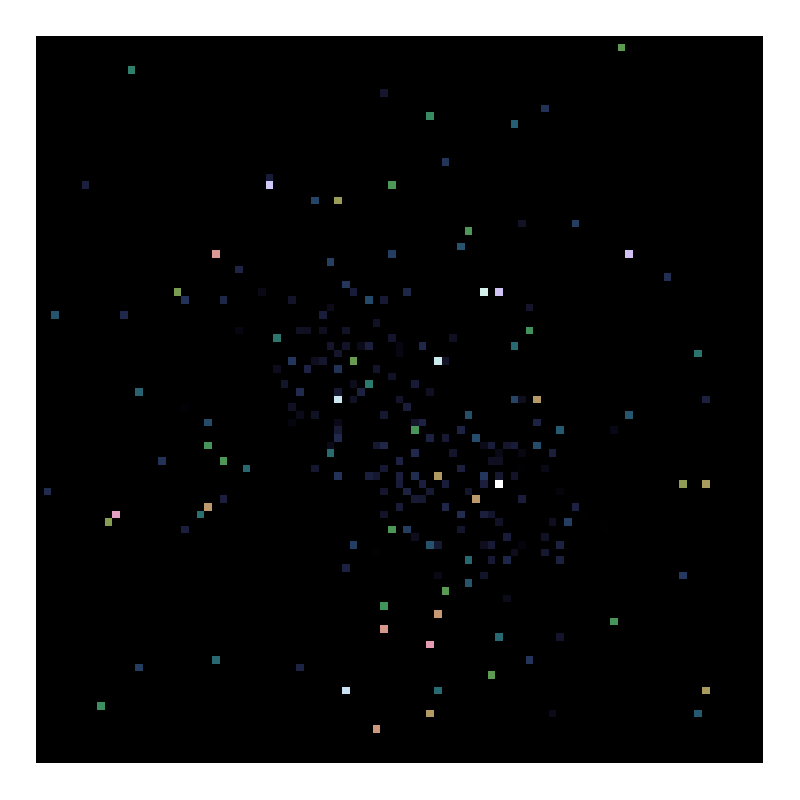
\includegraphics[width=1.00\linewidth, clip, trim= 0.25in 0.25in 0.25in 0.25in]{./chapters/05.pcdm/randomProblem/random_1k_block1.png}
		\caption{8k iterations}
		\label{pcdm:adaption:randomProblem:block11}
	\end{subfigure}
	\begin{subfigure}[b]{0.245\linewidth}
		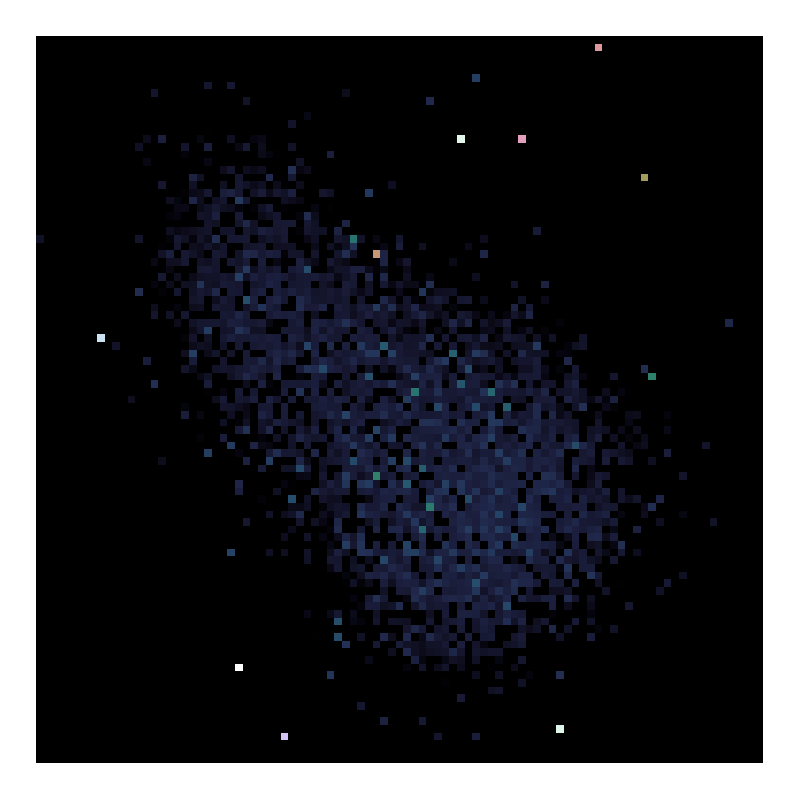
\includegraphics[width=1.00\linewidth, clip, trim= 0.25in 0.25in 0.25in 0.25in]{./chapters/05.pcdm/randomProblem/random_10k_block1.png}
		\caption{80k iterations}
		\label{pcdm:adaption:randomProblem:block12}
	\end{subfigure}
		\begin{subfigure}[b]{0.245\linewidth}
		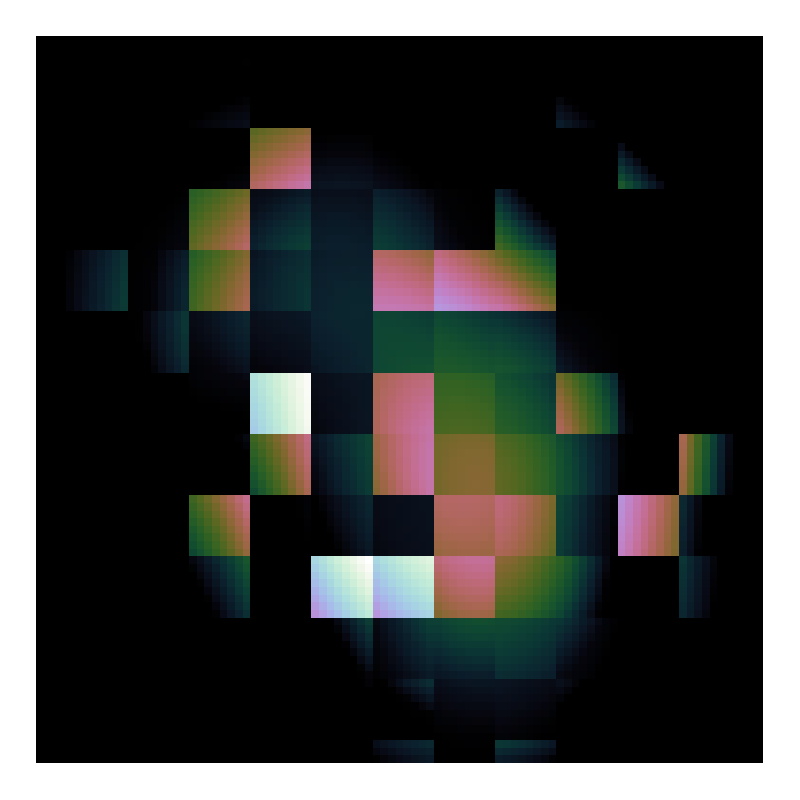
\includegraphics[width=1.00\linewidth, clip, trim= 0.25in 0.25in 0.25in 0.25in]{./chapters/05.pcdm/randomProblem/random_1k_block8.png}
		\caption{8k iterations, $8^2$ block}
		\label{pcdm:adaption:randomProblem:block81}
	\end{subfigure}
		\begin{subfigure}[b]{0.2405\linewidth}
		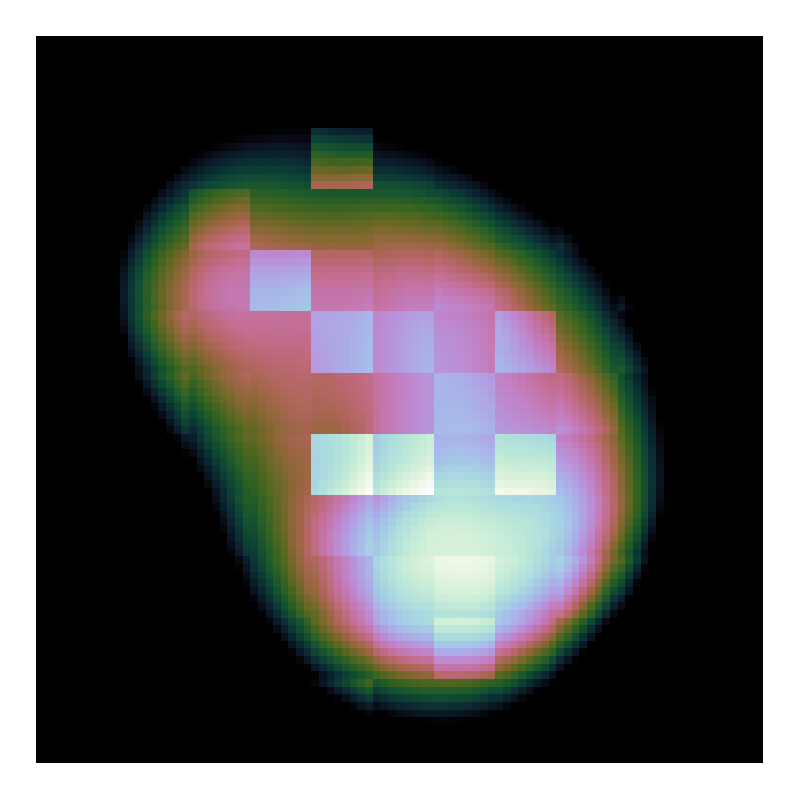
\includegraphics[width=1.00\linewidth, clip, trim= 0.25in 0.25in 0.25in 0.25in]{./chapters/05.pcdm/randomProblem/random_10k_block8.png}
		\caption{80k iterations, $8^2$ block}
		\label{pcdm:adaption:randomProblem:block82}
	\end{subfigure}
	\caption{Random parallel deconvolutions on the LMC N132D supernova remnant.}
	\label{pcdm:adaption:randomProblem}
\end{figure}

The Figure \ref{pcdm:adaption:randomProblem} shows the behaviour on the LMC observation. The reconstructions receive obvious artifacts from the random selection strategy. The blocks, which get selected in the first few iterations, keep their over-estimated values until we randomly select them again in later iterations. Other blocks in the neighborhood cannot be changed to a reasonable value until the algorithm has randomly selected the over-estimated blocks. That is why even after 80k iterations, the N132D supernova remnant gets only hinted at in Figure \ref{pcdm:adaption:randomProblem:block12}. Until the over-estimated blocks get selected again, the algorithm cannot do useful updates in that region.

This behavior is pronounced when we choose a block size of one pixel (i.e. we do not group pixels into blocks). Increasing the block size also increases our changes to select one of the over-estimated block again. But as we see in Figure \ref{pcdm:adaption:randomProblem:block82}, the same problem exists with larger block sizes, although less pronounced. After 80k iterations the N132D supernova remnant is visible, but a few random blocks still contain too much of the emission in that area.

The order in which we select blocks seems to be relevant in the deconvolution problem. A random selection strategy needs a prohibitive large number of iterations to converge. But we cannot simply switch out the selection strategy. The random selection strategy is at the core of the Parallel coordinate descent methods. Remember the ESO arises from the fact that we select $tau$ pixels uniformly at random. When we select $\tau$-pixels with a greedy strategy, we might break the ESO and may not converge.

To solve this behavior, we introduce the pseudo-random selection strategy:  We select a block at random, but greedily search in the neighborhood for the optimal block to optimize. The size of the neighborhood can be defined by the user. It is essentially a mix between a greedy and a random selection strategy. If we choose the neighborhood to be the whole image, we arrive at a greedy strategy. If we choose the neighborhood to be just one block, we are back at a random strategy. The mixture of the greedy and random strategy allows us to fix the problems with the pure random

We also introduced three heuristics that speed up the parallel deconvolution algorithm in practice: An active set heuristic, Restarting heuristic and a 'Minor' cycle.


\subsubsection{Active set heuristic}
The active set heuristic is typically used in cyclic coordinate descent: It chooses a subset of blocks, and optimizes the set until it converges. Then it chooses a  new set. We use the active set heuristic together with our pseudo-random selection strategy. A large portion of the blocks in the image will be zero. If we select blocks at pseudo-random, we are likely to select a block that will never contain non-zero values. The active set heuristic increases the likelihood that the pseudo-random strategy selects a relevant block. 

At the start of the parallel deconvolution algorithm, we iterate over all blocks. We add all blocks whose value can be changed to non-zero. During parallel iterations, the algorithm only selects blocks from the active set.

Note that the algorithm only adds blocks to the active set, which can be changed to a non-zero value at the start of deconvolution. Over several iterations, there may be blocks that are not in the active set, but are part of the optimal solution. This is remedied with a restarting heuristic.


\subsubsection{Restarting heuristic}
In accelerated gradient methods, like APPROX or (F)ISTA, restarting the acceleration can lead to a significant speedup\cite{fercoq2016restarting}. In our accelerated variant, restarting means we reset the acceleration variable $theta$ restart with the deconvolution, using the intermediate solution from the last iteration. Our accelerated deconvolution algorithm uses an active set. If we detect that important blocks are missing from the active set, we want to restart the deconvolution with a new active set. 

We implemented two restarting heuristics: One heuristic is based on Glasmachers et al.\cite{glasmachers2014coordinate} and restarts the algorithm when the acceleration likely benefits from it. The other heuristic was developed by us and restarts the when the active set is likely to be missing blocks. In our tests, we always needed to restart due to the active set, and never due to the heuristic by Glasmachers.

Our own restarting heuristic is based on the following idea: When the parallel deconvolutions start to converge before the currently best greedy step, we restart the algorithm with a new active set.

We introduce a new loop for the active set iteration. For each active set iteration, we execute several parallel deconvolution steps. For example, a single active set iteration may include 1000 parallel deconvolutions for each processor, running for $\tau * 1000$ iterations in total. Each processor updates the gradient maps and the reconstructed image asynchronously. We assume that after each active set iteration, we have landed at least once on the block that the greedy algorithm would have chosen in a single iteration.

At the end of each active set iteration, we check whether the parallel accelerated iterations converge faster than the currently best greedy step. If it does, we restart the parallel algorithm with a new active set.

\begin{lstlisting}
...
do
	lastMaxDiff = GetGreedyMaxBlockDiff(gradientsMapExplore, xExplore)
	parallelDiffFactor = 0
	for activeSetIteration in activeSetIterations
		
		//concurrent iterations
		maxParallelDiff = 0
		parallel for
			...
			diffBlock = optimalBlock - oldBlock
			...
			
			if(maxParallelDiff < diffBlock)
				maxParallelDiff = diffBlock
				
		//restarting heuristic
		if(parallelDiffFactor = 0)
			parallelDiffFactor = lastMaxDiff / maxParallelDiff
		
		currentMaxDiff = GetGreedyMaxBlockDiff(gradientsMapExplore, xExplore)
		activeSetInvalid = lastAbsMax / maxParallelDiff > parallelDiffFactor * 2
		activeSetInvalid = activeSetInvalid | currentMaxDiff > lastAbsMax & lastAbsMax / parallelDiffFactor > concurrentFactor
		if activeSetInvalid
			Restart()
			parallelDiffFactor = 0
		lastMaxDiff = currentMaxDiff
	..
while maxAbsDiff  < epsilon
\end{lstlisting}

After the first active set iteration, we check how close the maximum parallel update is to the best greedy step. The ratio of maximum greedy update and maximum parallel update should stay similar over the course of the algorithm, if the active set is valid. If the active set invalid, if it is missing important blocks, the algorithm will encounter ever smaller values for $maxParallelDiff$, while $lastMaxDiff$ does not decrease significantly over the active set iterations. In that case, the ratio between $lastMaxDiff / maxParallelDiff$ sharply increases, and we restart the algorithm.

We have two similar conditions on which we flag the active set as invalid. If the ratio of $lastMaxDiff / maxParallelDiff$ is twice as big as the ratio of the first active set iteration, we restart the algorithm. The second condition is based on the observation that the $currentMaxDiff$ may increase from active set iteration to active set iteration. In this case, we are likely missing important blocks in the active set and we restart more aggressively: If the ratio $lastMaxDiff / maxParallelDiff$ bigger than the ratio of the first active set iteration.


\subsubsection{Re-introduction of a 'Minor' cycles}
As we will demonstrate in the next section, the parallel coordinate descent deconvolution algorithm benefits significantly from our $PSF$ approximation. The drawback of our $PSF$ approximation is that it needs more major cycles to converge. We re-introduce a similar minor cycle to the Clark CLEAN algorithm \cite{clark1980efficient}, and reduce the number of necessary major cycles.

The CLEAN algorithm developed by Clark also uses only a fraction of the $PSF$ during CLEAN deconvolutions. After a number of iterations, the residuals of the Clark algorithm are inaccurate, and it resets the residuals with the full $PSF$.

We use a similar idea: We run our parallel coordinate descent deconvolution algorithm, and retrieve the intermediate solution. We then decide whether we reset the residuals using the full $PSF$ (the 'minor' cycle), or we use the major cycle.

Resetting the residuals with the full $PSF$ is done as follows:

\begin{lstlisting}
residuals = iFFT(Gridding(visibilities))  	//Major cycle
x = deconvolve(residuals, Cut(PSF)) 		//Deconvolve with approximate PSF
residuals_minor = residuals - iFFT(FFT(x) * FFT(PSF))
\end{lstlisting}

We convolve the intermediate solution $x$ with the $PSF$ in Fourier space, and subtract the result from the original residuals from the major cycle. This allows us to use fewer major cycles when we use an aggressive $PSF$ approximation.

The question only question that remains is, when to use a major cylce or a 'minor' cycle. Remember from Section \ref{gradients}, we introduced a heuristic based on the $PSF$ sidelobe: When we deconvolve using only a fraction of the full $PSF$, we leave sidelobes in the residual image. In each major cycle, we can only run the deconvolution algorithm up to a certain point, before we include $PSF$ sidelobes in the reconstructed image. 

In Section \ref{gradients} solved this by estimating a minimum regularization parameter $\lambda$ for each major cycle. Now with the addition of a 'minor' cycle, we use the same heuristic twice: We have two minimum regularization parameters, $\lambda_{minor}$ and $\lambda_{major}$. We use the minor cycle, as long as  $\lambda_{minor}$ is larger than  $\lambda_{major}$. Otherwise, we start a new major cycle. In total, the major and 'minor' cycle for our parallel coordinate descent algorithm is implemented as follows:

\begin{lstlisting}
residualVis = visibilities
x = new Array[,]

for each cycle in Range(0, maxMajorCycles)
	residuals = iFFT(Gridding(residualVis))
	residualsMinor = residuas
	
	lambdaMajor = Estimate(residuals, PSF, 2)
	lambdaMinor = 0
	
	do
		lambdaMinor = Estimate(residualsMinor, PSF, psfFraction)
		lambdaMinor = Max(lambdaMinor, lambdaMajor)
		
		x_current = deconvolve(residuals, Cut(PSF, psfFraction))
		x + = x_current
		residuals_minor = residuals - iFFT(FFT(x) * FFT(PSF))
	while(lambdaMajor < lambdaMinor)
	
	modelVis = DeGridding(FFT(x))
	residualVis = visibilities - modelVis
\end{lstlisting}

Estimating $\lambda_{minor}$ is identical to the heuristic developed in Section \ref{gradients}. We use the maximum sidelobe of the $PSF$ which is not contained in the cutout used for deconvolution. Estimating $\lambda_{major}$ is more difficult: In theory, we use the full $PSF$, and do not have a sidelobe outside the cutout. However, we also know that the full $PSF$ is only an approximation (remember: the $w$-term changes the $PSF$ slightly for all pixels in the image). For the parameter $\lambda_{major}$, we simply use the maximum sidelobe outside of the $\frac{1}{2}$ cutout.


\subsection{Tests on the LMC Observation}\label{pcdm:results}
We have shown the parallel coordinate descent algorithm in two variants: With gradient acceleration and without. We developed several heuristics, which includes a set of tuning parameters. In this section, we test our parallel coordinate descent algorithm on the MeerKAT LMC observation. We test the tuning parameters, and show how much our algorithm benefits from the $PSF$ approximation method.

In this test, we measure the wall-clock time of only the deconvolution. The wall-clock time of the Major- and 'Minor' cycle are excluded. Again, we calculate the value of the objective function. We compare different parameters of our parallel coordinate descent algorithm, trying to get the shortest convergence time.

\subsubsection{$PSF$ approximation}
First, we test the effect of our $PSF$ approximation method. We test different $PSF$ cutouts of our parallel coordinate descent algorithm with gradient acceleration. We use $\tau = 8$ processors with our asynchronous implementation.

Figure \ref{pcdm:results:psf} shows the result of our parallel coordinate descent algorithm with different $PSF$ fractions, combined with the ESO and the total seconds needed to converge. The $y$-axis shows the objective value, and the $x$-axis shows the elapsed seconds. Note that the axis of the figure are logarithmic. The 'kinks' in the lines are due to either the Major or the 'Minor' cycle resetting the residuals (remember: we do not include the wall-clock time of the Major or 'Minor' cycle in this test).

\begin{figure}[h]
	\centering
	\begin{subfigure}{0.6\linewidth}
		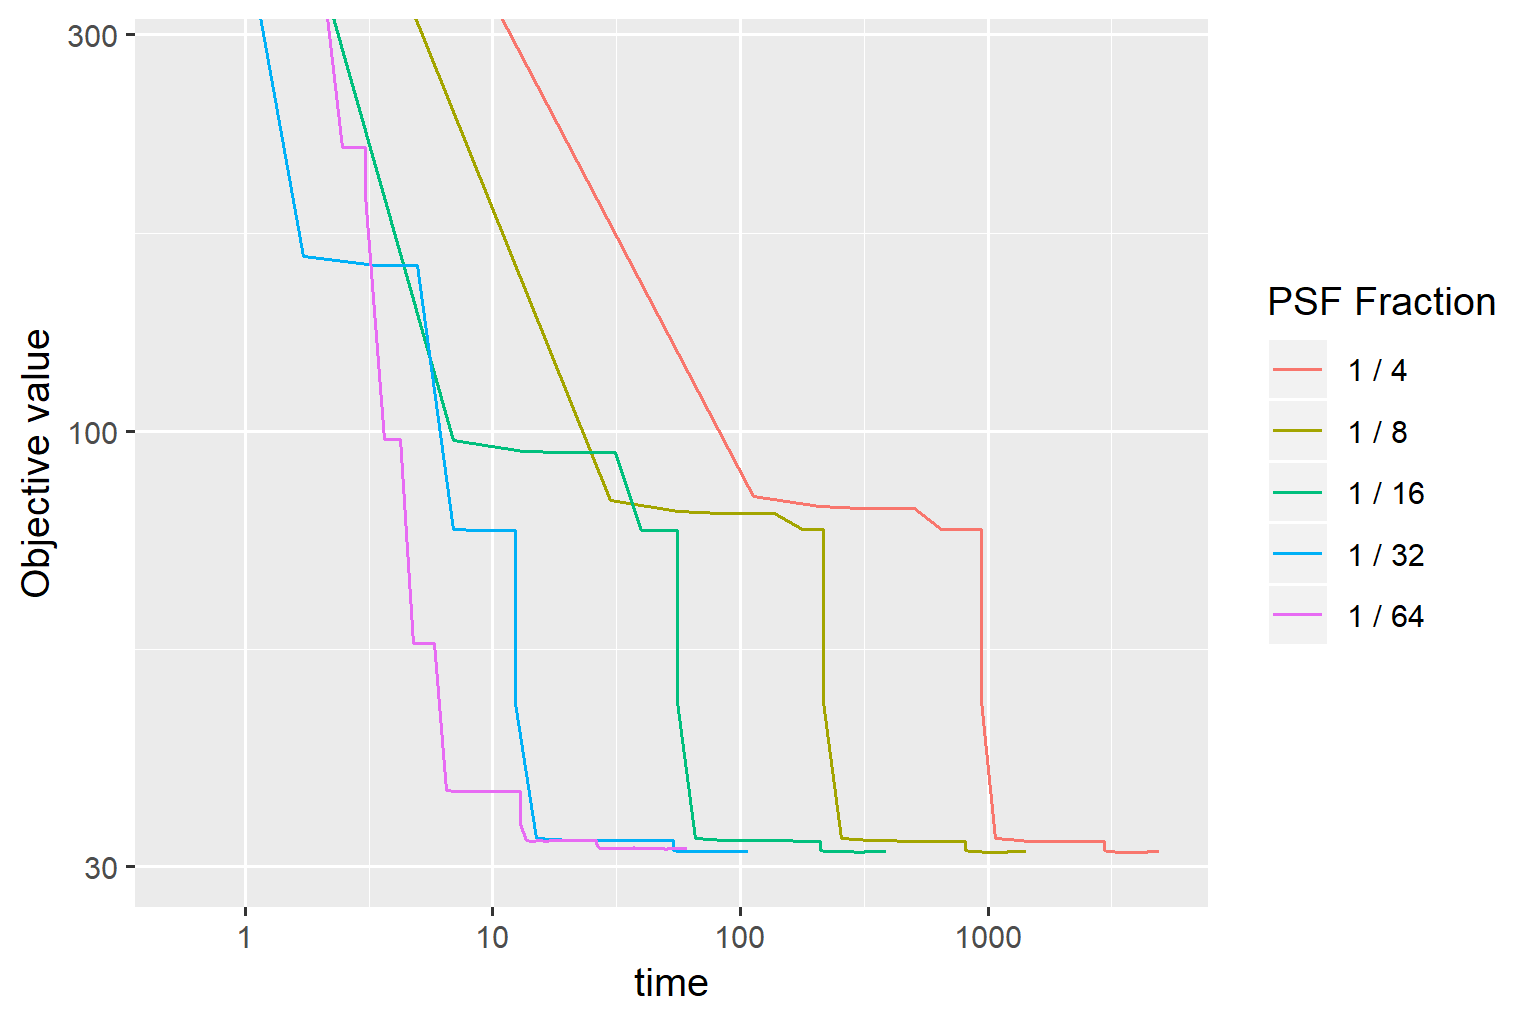
\includegraphics[width=1.0\linewidth]{./chapters/05.pcdm/parameters/psfSize.png}
	\end{subfigure}
	\begin{subfigure}{0.35\linewidth}
		\begin{tabular}{c | c | c}
			PSF & ESO & Total seconds \\ \hline
			1 / 4 & 1.437 & 4941 \\
			1 / 8 & 1.109 & 1433 \\
			1 / 16 & 1.027 & 390 \\
			1 / 32 & 1.007 & 108 \\
			1 / 64 & 1.002 & 61 \\
		\end{tabular}
	\end{subfigure}
	\caption{Convergence times with $PSF$ approximation}
	\label{pcdm:results:psf}
\end{figure}

Clearly, the parallel coordinate descent algorithm benefits from our $PSF$ approximation method. If we use $\frac{1}{32}$ of the full $PSF$, the parallel coordinate descent algorithm spends a total of 108 seconds in to deconvolve the image. For comparison, the serial coordinate descent algorithm with $PSF$ approximation takes roughly 1400 seconds, or 23 minutes.

As expected, with increasing $PSF$ approximation, we get an ESO which is ever closer to 1. Remember: An ESO of 1 means that each processor in the parallel coordinate descent algorithm can has the same step size as the serial coordinate descent algorithm. With an approximation of $\frac{1}{32}$ and 8 parallel processors, the ESO is only marginally larger than 1. This suggests that the parallel coordinate descent algorithm may be sped up further with additional processors.

Note that the speedup from fraction $\frac{1}{4}$ to $\frac{1}{8}$ is roughly a factor of $3.5$. The same holds true for the speedup of $\frac{1}{8}$ to $\frac{1}{16}$, and $\frac{1}{16}$ to $\frac{1}{32}$. The $PSF$ cutout from  $\frac{1}{8}$ to  $\frac{1}{16}$ four times fewer pixels. This suggest the speedup may be due to the reduced conflicts in the asynchronous update of the gradient map. With a smaller $PSF$ we reduce the change of several threads updating the same location in the gradient map, and we spend more time in the deconvolution itself.

For the rest of this project, we will use a $PSF$ approximation of $\frac{1}{32}$ for the parallel coordinate descent algorithm. The $\frac{1}{64}$ approximation is faster in this tests, but needs more 'Minor' cycles (Which were excluded from the wall-clock time). Including the time spent in the 'Minor' cycle, the $\frac{1}{32}$ approximation is the fastest overall.


\subsubsection{Block size}
The parallel coordinate descent algorithm can group several pixels in blocks, and optimize the blocks of pixels in parallel. It is not clear if grouping the pixels in blocks results in shorter convergence times. We test different block sizes in Figure \ref{pcdm:results:block}, all using the same $PSF$ approximation of $\frac{1}{32}$. We tested out block size of $1^2$ (every block contains a single pixel) up to a block size of $8^2$:

\begin{figure}[h]
	\centering
	\begin{subfigure}{0.6\linewidth}
		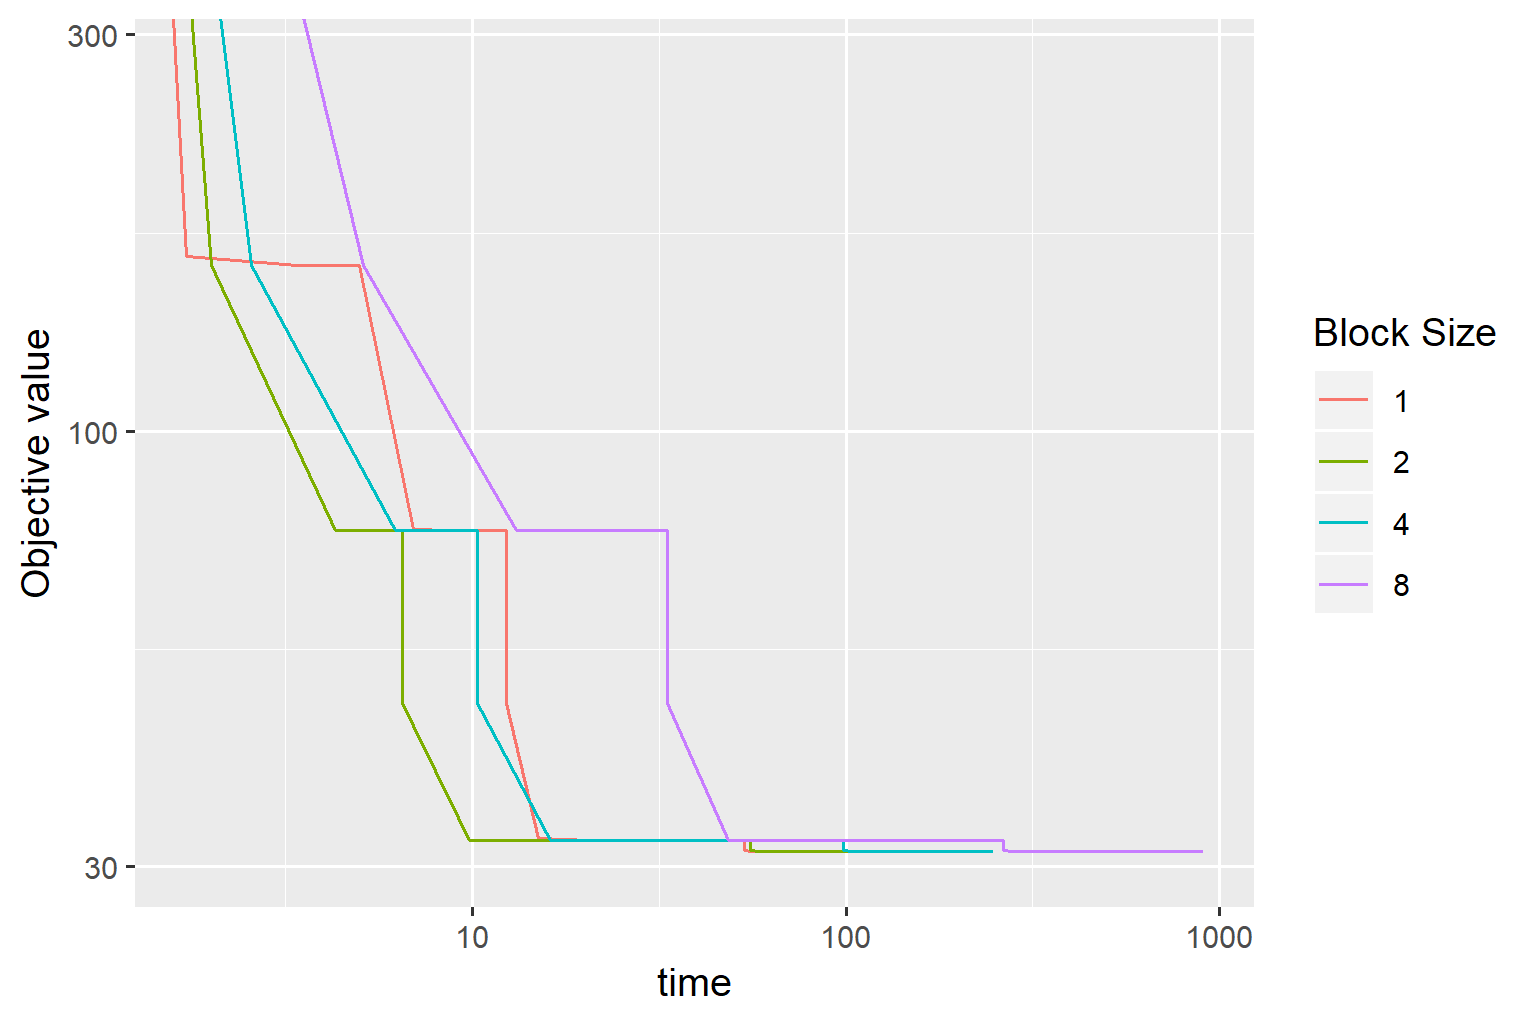
\includegraphics[width=1.0\linewidth]{./chapters/05.pcdm/parameters/blockSize.png}
	\end{subfigure}
	\begin{subfigure}{0.35\linewidth}
		\begin{tabular}{c | c}
			Block Size & Total seconds \\ \hline
			$1^2$ & 108 \\
			$2^2$ & 103 \\
			$4^2$ & 248 \\
			$8^2$ & 905 \\
		\end{tabular}
	\end{subfigure}
	\caption{Convergence times with different block sizes}
	\label{pcdm:results:block}
\end{figure}

The larger block sizes of $4^2$ and $8^2$ are significantly slower to converge than a block size of $1^2$. Only a block size of $2^2$ is slightly faster. Interestingly though, the parallel coordinate descent algorithm is faster to arrive at intermediate results with the block sizes $2^2$ and $4^2$. This suggests that the parallel coordinate descent algorithm may benefit starting out from larger block sizes, and gradually reducing the block size over several major cycle iterations.

However, two factors lead to the decision to simply use a block size of $1^2$ for all major cycle iterations: First, the block size is likely connected to the image resolution. An effective heuristic that starts with larger blocks may become difficult to develop for general observations. Secondly, the parallel coordinate descent implementation becomes more complicated when it has to account for different block sizes. An implementation with a block size of only $1^2$ is shorter and simpler.

For the rest of this project, we use a block size of $1$, meaning every thread is minimizing a single pixel.


\subsubsection{Pseudo-random strategy}
We discussed in Section \ref{pcdm:adaption}, a random block selection strategy seems to perform badly on the deconvolution problem. We created the pseudo-random strategy, which selects a block at random, but searches in it's neighborhood for the optimal block to optimize. It is a mixture between a random and a greedy selection strategy.

But the pseudo-random strategy introduces a new tuning parameter, which we call the 'search percentage'. A search percentage of 0 says that after a random block has been selected, we search 0\% of the neighboring blocks in the active set. It is identical to a pure random selection strategy. A search percentage of 1.0 says that after a random block has been selected, we search 100\% of its neighbors in the active set. For example, if we have 256 blocks with 8 threads, a search percentage of 1.0 selects a random block and looks at 32 blocks in its neighborhood. A search percentage of 100\% is identical to a greedy strategy, where each thread searches its part of the active set.

Our parallel coordinate descent algorithm needs a search percentage larger than 0. We compare different search percentages in Figure \ref{pcdm:results:search}.

\begin{figure}[h]
	\centering
	\begin{subfigure}{0.6\linewidth}
		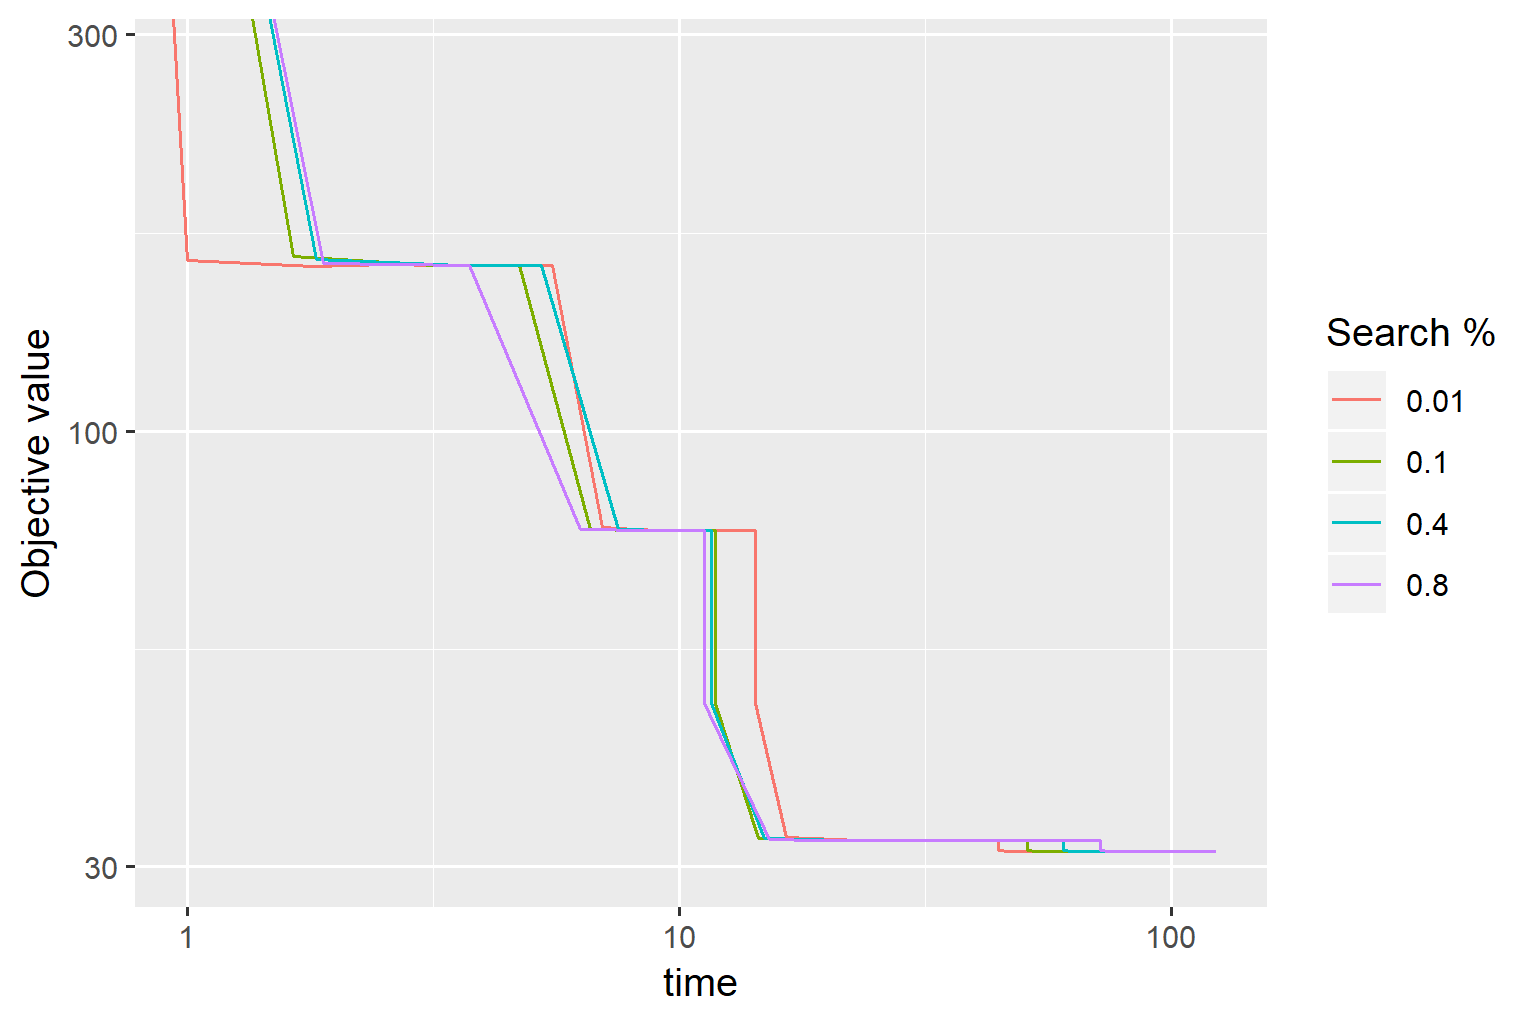
\includegraphics[width=1.0\linewidth]{./chapters/05.pcdm/parameters/searchPercent.png}
	\end{subfigure}
	\begin{subfigure}{0.35\linewidth}
		\begin{tabular}{c | c}
			Search Percentage & Total seconds \\ \hline
			0.01 & 110 \\
			0.1 & 106 \\
			0.2 & 104 \\
			0.4 & 112 \\
			0.8 & 134 \\
		\end{tabular}
	\end{subfigure}
	\caption{Convergence times with different search percentages.}
	\label{pcdm:results:search}
\end{figure}

And it is a tiny fraction. A lot less communication cost. Close to random, but not quite.


\subsubsection{Acceleration}
Lastly, we test whether the parallel coordinate descent algorithm is faster with or without gradient acceleration. The accelerated variant needs two versions of the gradient map, which get updated asynchronously with compare-exchange operations. Figure \ref{pcdm:results:acc} compares the accelerated and non-accelerated parallel coordinate descent algorithm.

\begin{figure}[h]
	\centering
	\begin{subfigure}{0.6\linewidth}
		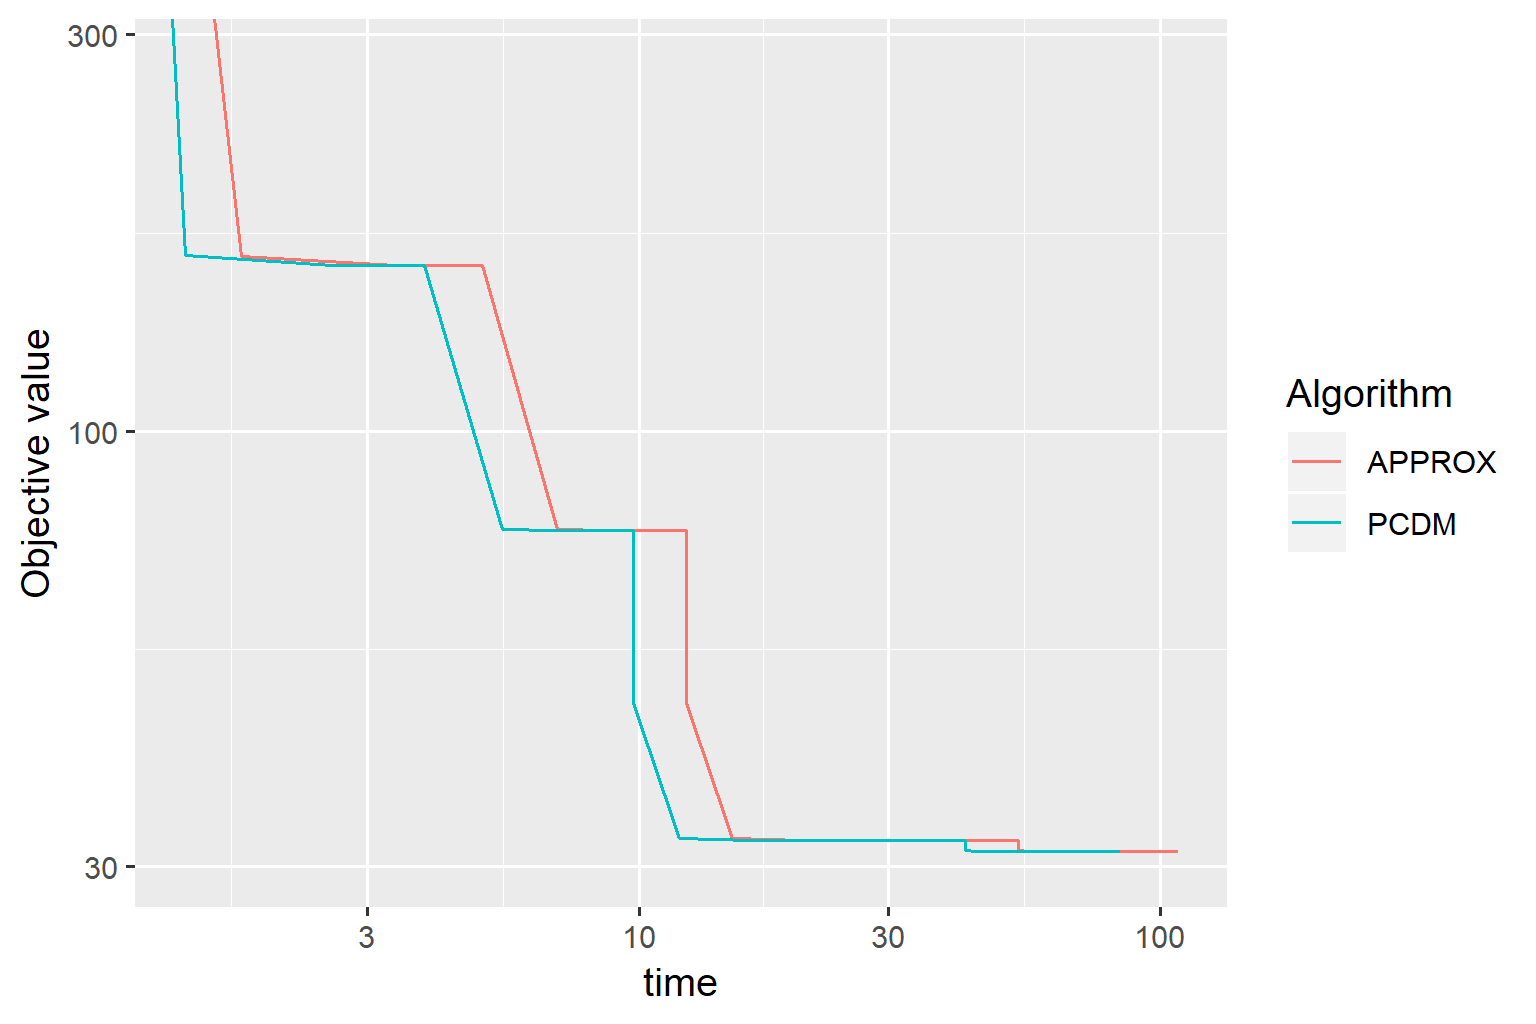
\includegraphics[width=1.0\linewidth]{./chapters/05.pcdm/parameters/acceleration.png}
	\end{subfigure}
	\begin{subfigure}{0.35\linewidth}
		\begin{tabular}{c | c}
			Method & Total seconds \\ \hline
			With Acceleration & 108 \\
			Without Acceleration & 84 \\
		\end{tabular}
	\end{subfigure}
	\caption{Convergence time with or without gradient acceleration.}
	\label{pcdm:results:acc}
\end{figure}

The accelerated variant is significantly slower in every part of the algorithm. Our hypothesis is that the two gradient maps necessary for the acceleration also increase the cost of synchronization.

Furthermore the accelerated variant has additional run time costs which were not measured in this test: It has to create a copy of the gradient map and the reconstructed image for the acceleration. Meaning this test shown in Figure \ref{pcdm:results:acc} is biased in favor of the accelerated variant, yet it is still slower.


\subsection{Comparison to the serial coordinate descent algorithm}
In the previous section, we tested various tuning parameters of the parallel coordinate descent algorithm. In this section, we compare the serial coordinate descent algorithm with the final, simplified parallel coordinate descent algorithm.

We took the lessons from the tests and implemented a simplified parallel coordinate descent algorithm. It does not use gradient acceleration, and cannot group pixels into blocks. Each thread can only minimize a single pixel in parallel in each iteration. As we will see shortly, the simplified parallel coordinate descent implementation is significantly faster than the previous implementation.

In this test, we compare the wall-clock time spent on the deconvolution algorithm. The time we measure here does not include the Major cycle. For the parallel coordinate descent algorithm, this means we also measure the time spent in the 'Minor' cycle for the parallel coordinate descent algorithm (which was excluded in the previous tests).

We use the same hardware as in the tests of Section \ref{results:LMC}. The table \ref{pcdm:comp:table} shows the comparison between the serial and parallel coordinate descent algorithm. The parallel coordinate descent algorithm achieved a speedup factor of roughly $20$. While the serial coordinate descent algorithm takes over 20 minutes to deconvolve the image, the parallel coordinate descent algorithm takes less than two minutes in total.
%hardware

\begin{table} [h]
	\centering
	\begin{tabular}{c | c | c | c | c}
		Algorithm &  $PSF$ Fraction & Major Cycles & Total Seconds in Deconvolution & Speedup factor\\ \hline
		Serial CD & $\frac{1}{16}$ & 4 & 1486 & --\\
		Parallel CD & $\frac{1}{32}$ & 5 & 75 & $\approx 20$ \\
	\end{tabular}
	\caption{Speedup comparison of the serial and parallel coordinate descent algorithm. Both algorithms were compared on an Intel Xeon E3-1505M with 8 logical cores.}
	\label{pcdm:comp:table}
\end{table}

This parallel coordinate descent implementation is even faster than the implementation tested in the previous Section \ref{pcdm:results}. This implementation is simpler because it does not account for different block sizes. Each processor deconvolves a single pixel in parallel. The simplification leads to another decrease in wall-clock time.

Comparison to CLEAN.

Note however that the serial coordinate descent requires one less major cycle.

Faster than even the previous parallel coordinate descent implementation. Simplified because we do not need to account for blocks of pixels.
But needs a major cycle more than the serial coordinate descent algorithm.
What was measured: Including the 'Minor' cycle.
		
Fastest variants of both. Serial coordinate descent


Compare the images from serial coordinate descent to the parallel coordinate descent, shown in Figure \ref{pcdm:comparison:figure}.
\begin{figure}[h]
	\centering
	\begin{subfigure}{0.4\linewidth}
		\centering
		Serial CD
		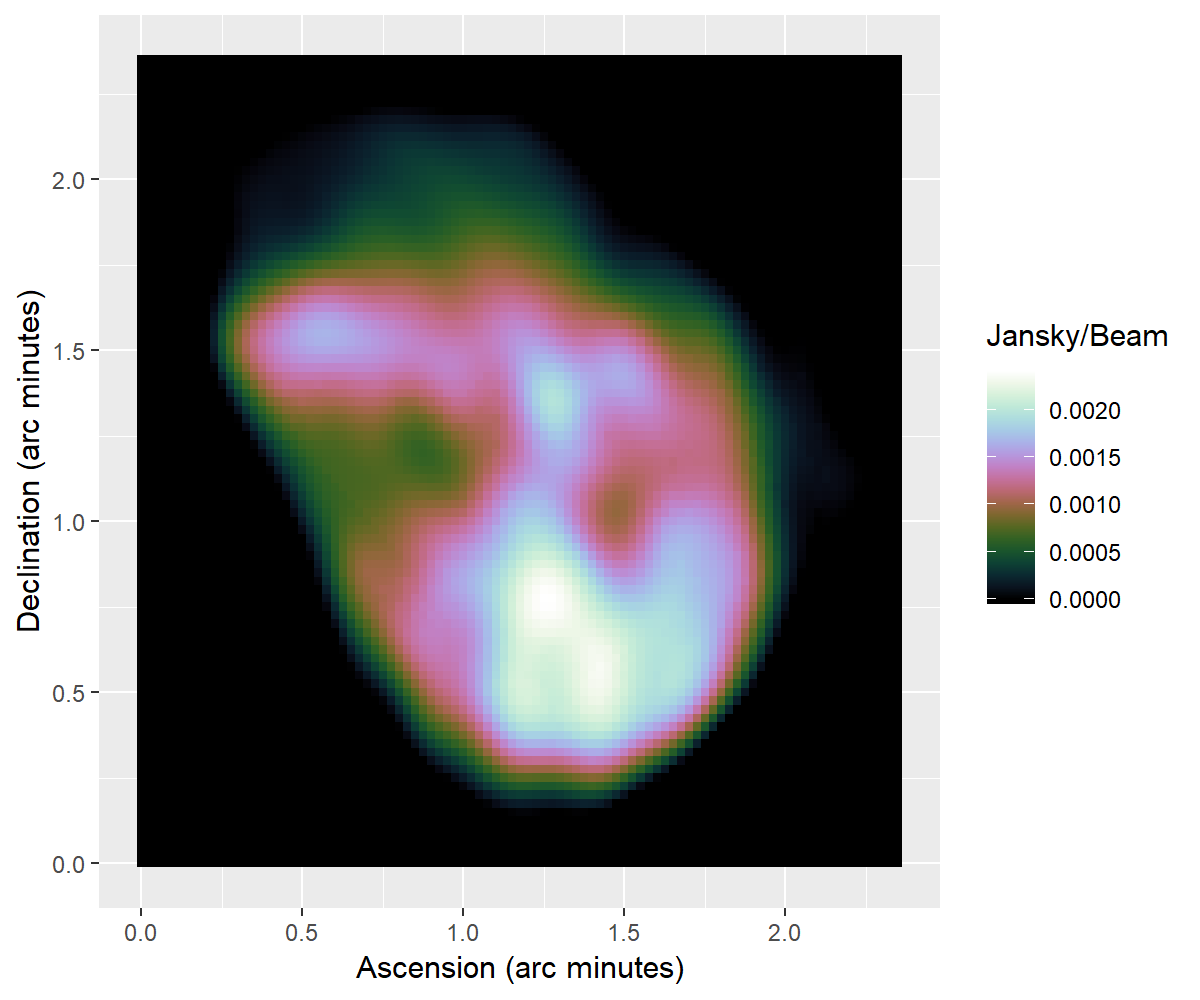
\includegraphics[width=1.0\linewidth]{./chapters/05.pcdm/comparison/SerialCD-N132.png}
	\end{subfigure}
	\begin{subfigure}{0.4\linewidth}
		\centering
		Parallel CD
		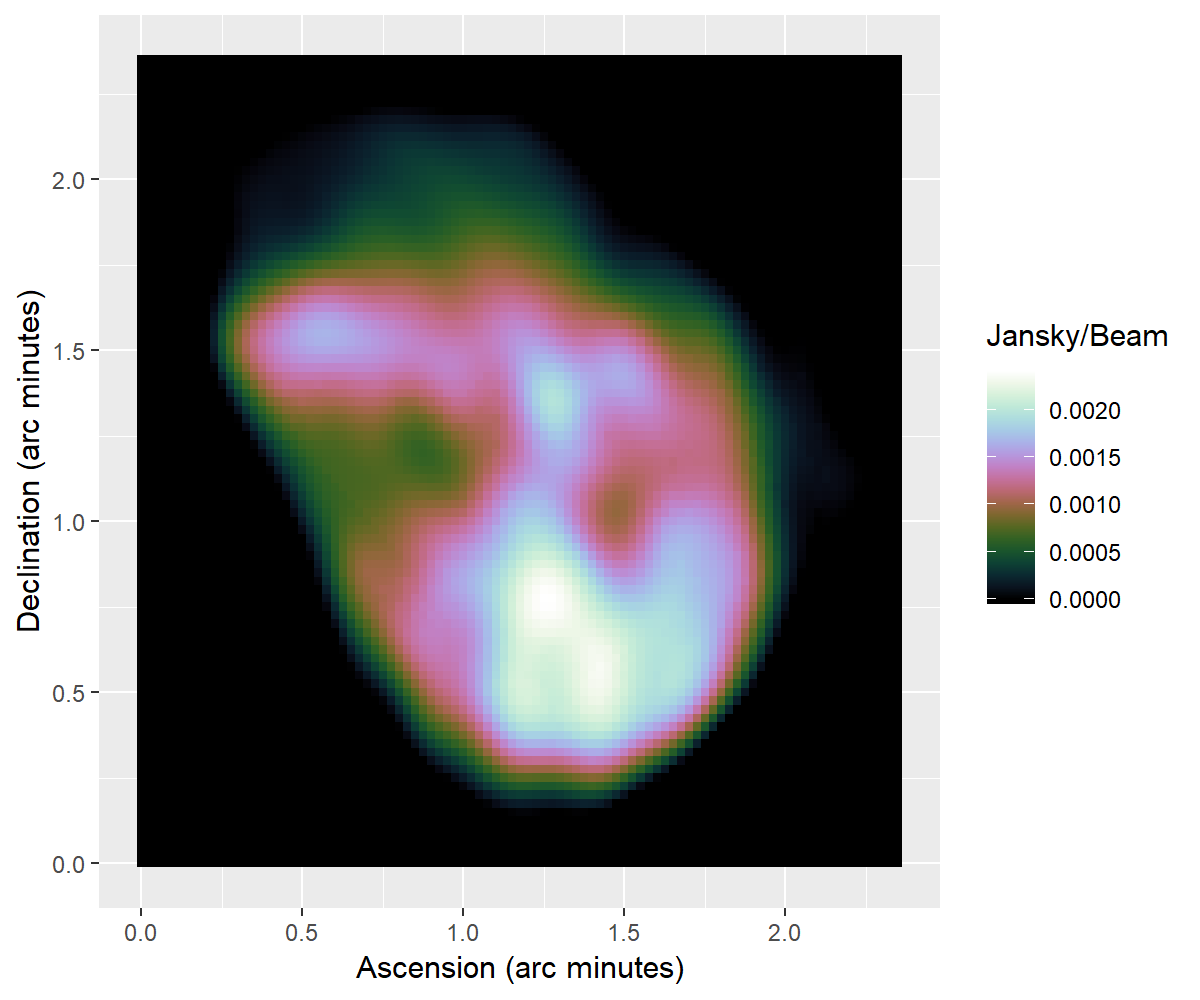
\includegraphics[width=1.0\linewidth]{./chapters/05.pcdm/comparison/SerialCD-N132.png}
	\end{subfigure}
	\\
	\begin{subfigure}{0.4\linewidth}
		\centering
		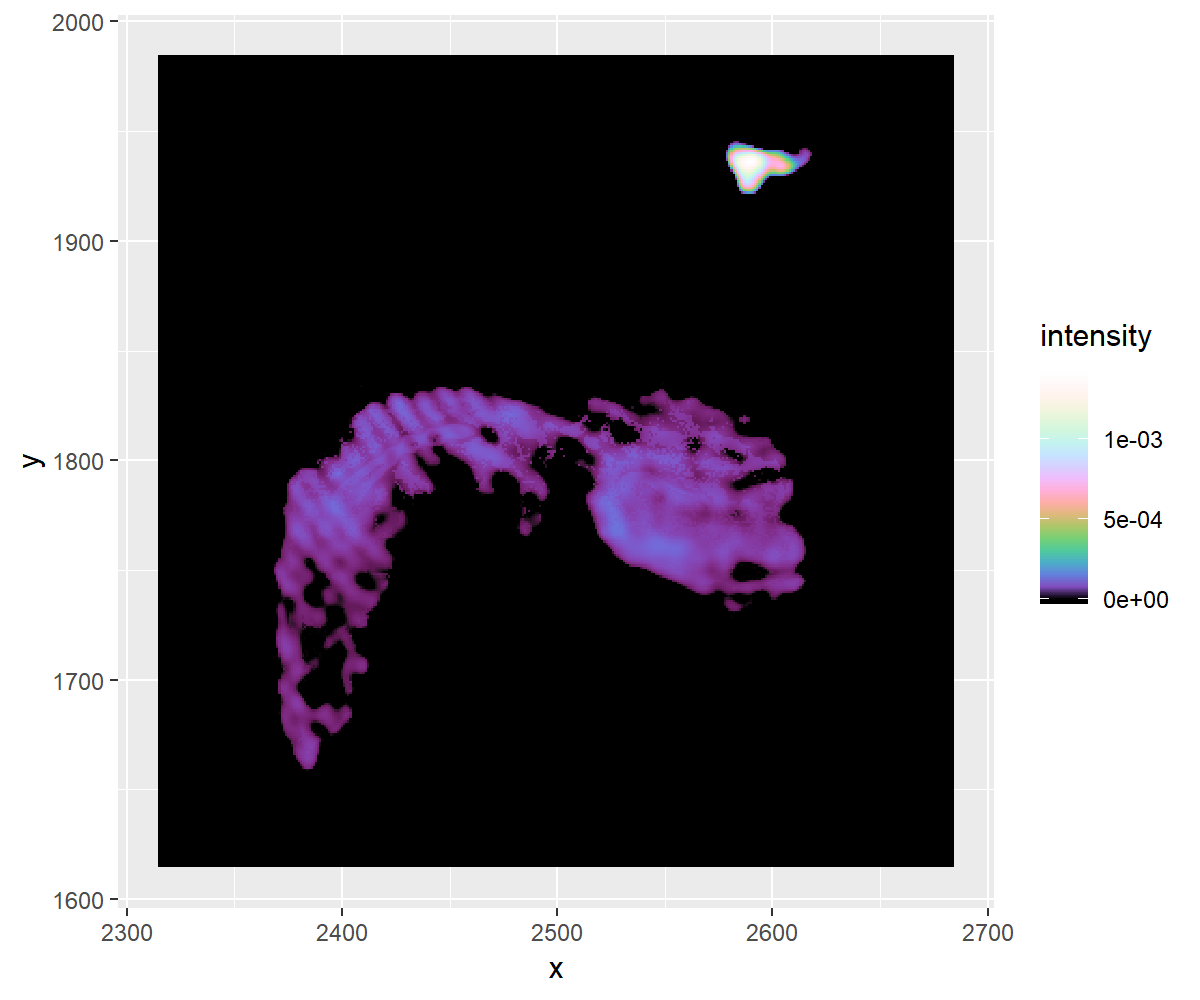
\includegraphics[width=1.0\linewidth]{./chapters/05.pcdm/comparison/SerialCD-Calibration.png}
	\end{subfigure}
	\begin{subfigure}{0.4\linewidth}
		\centering
		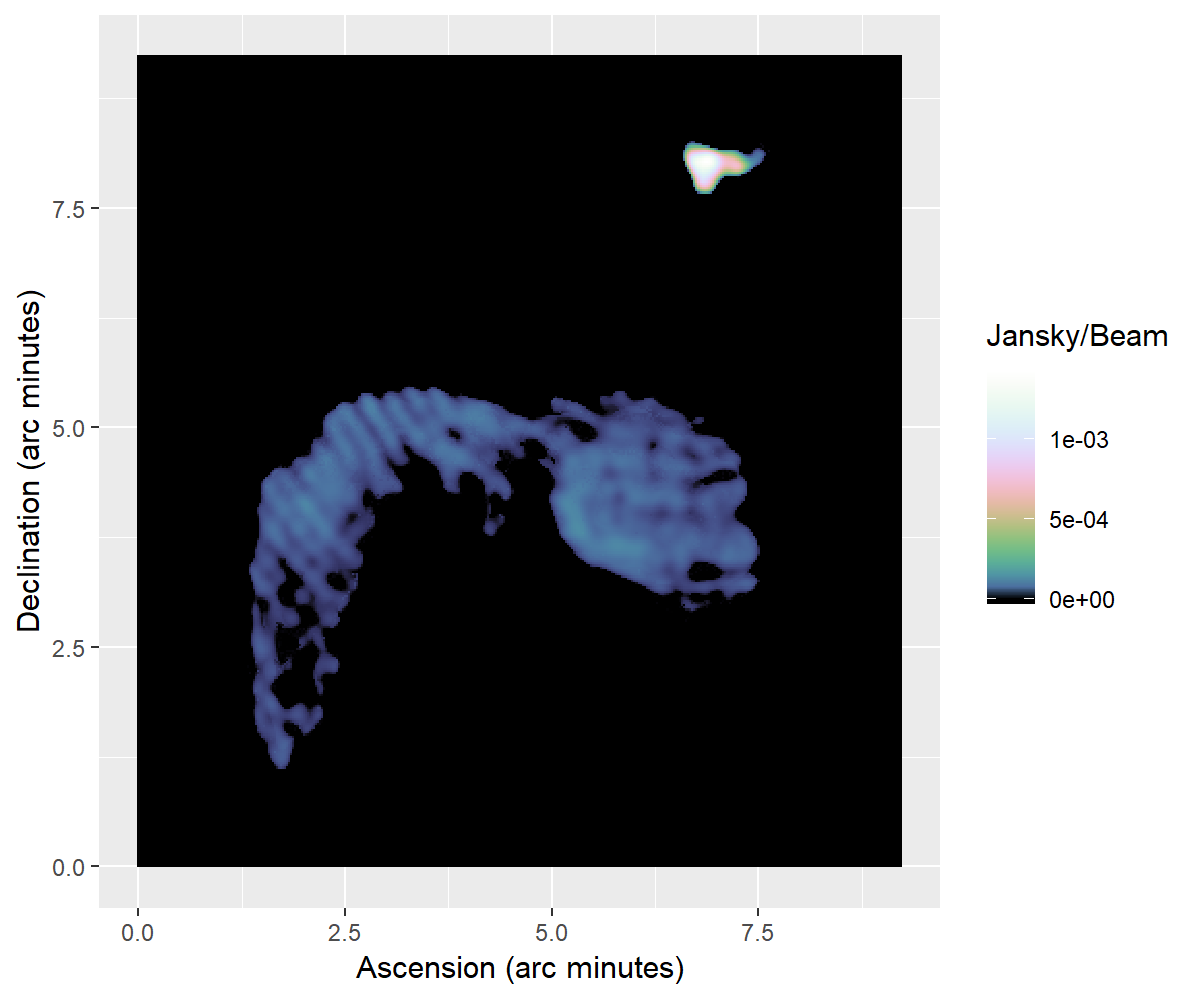
\includegraphics[width=1.0\linewidth]{./chapters/05.pcdm/comparison/PCDM-Calibration.png}
	\end{subfigure}

	\caption{Comparison of the serial and parallel coordinate descent reconstruction of the LMC observation.}
	\label{pcdm:comparison:figure}
\end{figure}


Acceleration factor

images


\subsection{Scalability of the parallel coordinate descent algorithm}
How many processors can we realistically use. At what point does the $ESO$ get too small.




